% Options for packages loaded elsewhere
\PassOptionsToPackage{unicode,linktoc=all}{hyperref}
\PassOptionsToPackage{hyphens}{url}
\PassOptionsToPackage{dvipsnames,svgnames,x11names}{xcolor}
%
\documentclass[
  a4paper,
]{article}
\usepackage{amsmath,amssymb}
\usepackage{iftex}
\ifPDFTeX
  \usepackage[T1]{fontenc}
  \usepackage[utf8]{inputenc}
  \usepackage{textcomp} % provide euro and other symbols
\else % if luatex or xetex
  \usepackage{unicode-math} % this also loads fontspec
  \defaultfontfeatures{Scale=MatchLowercase}
  \defaultfontfeatures[\rmfamily]{Ligatures=TeX,Scale=1}
\fi
\usepackage{lmodern}
\ifPDFTeX\else
  % xetex/luatex font selection
\fi
% Use upquote if available, for straight quotes in verbatim environments
\IfFileExists{upquote.sty}{\usepackage{upquote}}{}
\IfFileExists{microtype.sty}{% use microtype if available
  \usepackage[]{microtype}
  \UseMicrotypeSet[protrusion]{basicmath} % disable protrusion for tt fonts
}{}
\makeatletter
\@ifundefined{KOMAClassName}{% if non-KOMA class
  \IfFileExists{parskip.sty}{%
    \usepackage{parskip}
  }{% else
    \setlength{\parindent}{0pt}
    \setlength{\parskip}{6pt plus 2pt minus 1pt}}
}{% if KOMA class
  \KOMAoptions{parskip=half}}
\makeatother
\usepackage{xcolor}
\usepackage[margin=25mm]{geometry}
\usepackage{longtable,booktabs,array}
\usepackage{calc} % for calculating minipage widths
% Correct order of tables after \paragraph or \subparagraph
\usepackage{etoolbox}
\makeatletter
\patchcmd\longtable{\par}{\if@noskipsec\mbox{}\fi\par}{}{}
\makeatother
% Allow footnotes in longtable head/foot
\IfFileExists{footnotehyper.sty}{\usepackage{footnotehyper}}{\usepackage{footnote}}
\makesavenoteenv{longtable}
\usepackage{graphicx}
\makeatletter
\def\maxwidth{\ifdim\Gin@nat@width>\linewidth\linewidth\else\Gin@nat@width\fi}
\def\maxheight{\ifdim\Gin@nat@height>\textheight\textheight\else\Gin@nat@height\fi}
\makeatother
% Scale images if necessary, so that they will not overflow the page
% margins by default, and it is still possible to overwrite the defaults
% using explicit options in \includegraphics[width, height, ...]{}
\setkeys{Gin}{width=\maxwidth,height=\maxheight,keepaspectratio}
% Set default figure placement to htbp
\makeatletter
\def\fps@figure{htbp}
\makeatother
\usepackage{svg}
\setlength{\emergencystretch}{3em} % prevent overfull lines
\providecommand{\tightlist}{%
  \setlength{\itemsep}{0pt}\setlength{\parskip}{0pt}}
\setcounter{secnumdepth}{-\maxdimen} % remove section numbering
% definitions for citeproc citations
\NewDocumentCommand\citeproctext{}{}
\NewDocumentCommand\citeproc{mm}{%
  \begingroup\def\citeproctext{#2}\cite{#1}\endgroup}
\makeatletter
 % allow citations to break across lines
 \let\@cite@ofmt\@firstofone
 % avoid brackets around text for \cite:
 \def\@biblabel#1{}
 \def\@cite#1#2{{#1\if@tempswa , #2\fi}}
\makeatother
\newlength{\cslhangindent}
\setlength{\cslhangindent}{1.5em}
\newlength{\csllabelwidth}
\setlength{\csllabelwidth}{3em}
\newenvironment{CSLReferences}[2] % #1 hanging-indent, #2 entry-spacing
 {\begin{list}{}{%
  \setlength{\itemindent}{0pt}
  \setlength{\leftmargin}{0pt}
  \setlength{\parsep}{0pt}
  % turn on hanging indent if param 1 is 1
  \ifodd #1
   \setlength{\leftmargin}{\cslhangindent}
   \setlength{\itemindent}{-1\cslhangindent}
  \fi
  % set entry spacing
  \setlength{\itemsep}{#2\baselineskip}}}
 {\end{list}}
\usepackage{calc}
\newcommand{\CSLBlock}[1]{\hfill\break#1\hfill\break}
\newcommand{\CSLLeftMargin}[1]{\parbox[t]{\csllabelwidth}{\strut#1\strut}}
\newcommand{\CSLRightInline}[1]{\parbox[t]{\linewidth - \csllabelwidth}{\strut#1\strut}}
\newcommand{\CSLIndent}[1]{\hspace{\cslhangindent}#1}
\ifLuaTeX
\usepackage[bidi=basic]{babel}
\else
\usepackage[bidi=default]{babel}
\fi
\babelprovide[main,import]{british}
% get rid of language-specific shorthands (see #6817):
\let\LanguageShortHands\languageshorthands
\def\languageshorthands#1{}
% $HOME/.pandoc/defaults/latex-header-includes.tex
% Common header includes for both lualatex and xelatex engines.
%
% Preliminaries
%
% \PassOptionsToPackage{rgb,dvipsnames,svgnames}{xcolor}
% \PassOptionsToPackage{main=british}{babel}
\PassOptionsToPackage{english}{selnolig}
\AtBeginEnvironment{quote}{\small}
\AtBeginEnvironment{quotation}{\small}
\AtBeginEnvironment{longtable}{\centering}
%
% Packages that are useful to include
%
\usepackage{graphicx}
\usepackage{subcaption}
\usepackage[inkscapeversion=1]{svg}
\usepackage[defaultlines=4,all]{nowidow}
\usepackage{etoolbox}
\usepackage{fontsize}
\usepackage{newunicodechar}
\usepackage{pdflscape}
\usepackage{fnpct}
\usepackage{parskip}
  \setlength{\parindent}{0pt}
\usepackage[style=american]{csquotes}
% \usepackage{setspace} Use the <fontname-plus.tex> files for setspace
%
\usepackage{hyperref} % cleveref must come AFTER hyperref
\usepackage[capitalize,noabbrev]{cleveref} % Must come after hyperref
\let\longdivision\relax
\usepackage{longdivision}
% noto-plus.tex
% Font-setting header file for use with Pandoc Markdown
% to generate PDF via LuaLaTeX.
% The main font is Noto Serif.
% Other main fonts are also available in appropriately named file.
\usepackage{fontspec}
\usepackage{setspace}
\setstretch{1.3}
%
\defaultfontfeatures{Ligatures=TeX,Scale=MatchLowercase,Renderer=Node} % at the start always
%
% For English
% See also https://tex.stackexchange.com/questions/574047/lualatex-amsthm-polyglossia-charissil-error
% We use Node as Renderer for the Latin Font and Greek Font and HarfBuzz as renderer ofr Indic fonts.
%
\babelfont{rm}[Script=Latin,Scale=1]{NotoSerif}% Config is at $HOME/texmf/tex/latex/NotoSerif.fontspec
\babelfont{sf}[Script=Latin]{SourceSansPro}% Config is at $HOME/texmf/tex/latex/SourceSansPro.fontspec
\babelfont{tt}[Script=Latin]{FiraMono}% Config is at $HOME/texmf/tex/latex/FiraMono.fontspec
%
% Sanskrit, Tamil, and Greek fonts
%
\babelprovide[import, onchar=ids fonts]{sanskrit}
\babelprovide[import, onchar=ids fonts]{tamil}
\babelprovide[import, onchar=ids fonts]{greek}
%
\babelfont[sanskrit]{rm}[Scale=1.1,Renderer=HarfBuzz,Script=Devanagari]{NotoSerifDevanagari}
\babelfont[sanskrit]{sf}[Scale=1.1,Renderer=HarfBuzz,Script=Devanagari]{NotoSansDevanagari}
\babelfont[tamil]{rm}[Renderer=HarfBuzz,Script=Tamil]{NotoSerifTamil}
\babelfont[tamil]{sf}[Renderer=HarfBuzz,Script=Tamil]{NotoSansTamil}
\babelfont[greek]{rm}[Script=Greek]{GentiumBookPlus}
%
% Math font
%
\usepackage{unicode-math} % seems not to hurt % fallabck
\setmathfont[bold-style=TeX]{STIX Two Math}
\usepackage{amsmath}
\usepackage{esdiff} % for derivative symbols
% \renewcommand{\mathbf}{\symbf}
%
%
% Other fonts
%
\newfontfamily{\emojifont}{Symbola}
%

\usepackage{titling}
\usepackage{fancyhdr}
    \pagestyle{fancy}
    \fancyhead{}
    \fancyfoot{}
    \renewcommand{\headrulewidth}{0.2pt}
    \renewcommand{\footrulewidth}{0.2pt}
    \fancyhead[LO,RE]{\scshape\thetitle}
    \fancyfoot[CO,CE]{\footnotesize Copyright © 2006\textendash\the\year, R (Chandra) Chandrasekhar}
    \fancyfoot[RE,RO]{\thepage}
%
\usepackage{newunicodechar}
\newunicodechar{√}{\textsf{√}}
\usepackage {caption}
    \captionsetup{font={sf,stretch=1.4}}
\ifLuaTeX
  \usepackage{selnolig}  % disable illegal ligatures
\fi
\IfFileExists{bookmark.sty}{\usepackage{bookmark}}{\usepackage{hyperref}}
\IfFileExists{xurl.sty}{\usepackage{xurl}}{} % add URL line breaks if available
\urlstyle{sf}
\hypersetup{
  pdftitle={The Pi of Archimedes},
  pdfauthor={R (Chandra) Chandrasekhar},
  pdflang={en-GB},
  colorlinks=true,
  linkcolor={DarkOliveGreen},
  filecolor={Purple},
  citecolor={DarkKhaki},
  urlcolor={Maroon},
  pdfcreator={LaTeX via pandoc}}

\title{The Pi of Archimedes}
\author{R (Chandra) Chandrasekhar}
\date{2004-01-14 | 2024-07-10}

\begin{document}
\maketitle

\thispagestyle{empty}


\begin{quote}
This blog began life more than two decades ago, as part of a series of
lectures I delivered to very bright first-year engineering students at
an Australian university.

The number \(\pi\) (pronounced ``pie'') has been recognized from time
immemorial because its physical significance can be grasped easily: it
is the ratio of the circumference of a circle to its diameter. But who
would have thought that such an innocent ratio would exercise such
endless fascination because of the complexities it enfolds?

Not surprisingly, some high students I met recently wanted to know more
about \(\pi\). Accordingly, I have substantially recast and refreshed my
original presentation to better accord with the form and substance of a
blog. The online references have also been updated to keep up with a
rapidly changing Web.

My original intention was to write a single blog on \(\pi\). But because
I did not want it to become yet another overly long \emph{slog}, I have
decided to divide the material into two parts.

If there are any errors or omissions, please
\href{mailto:feedback.swanlotus@gmail.com}{email} me your feedback.
\end{quote}

\subsection{Circumference, diameter, and
π}\label{circumference-diameter-and-ux3c0}

The straight line or
\href{https://mathworld.wolfram.com/Geodesic.html}{geodesic} is the
shortest distance between any two points on a plane, sphere, or other
space. The circle is the
\href{https://en.wikipedia.org/wiki/Locus_(mathematics)}{locus}
traversed by a moving point that is
\href{https://en.wikipedia.org/wiki/Equidistant}{equidistant} from
another fixed point on a two-dimensional plane. It is the most
\href{https://mathworld.wolfram.com/Symmetry.html}{symmetrical} figure
on the plane. The
\href{https://en.wikipedia.org/wiki/Diameter}{diameter} is the name
given both to any straight line passing through the centre of the
circle---intersecting it at two points---as well as to its length. When
we divide the \href{https://en.wikipedia.org/wiki/Perimeter}{perimeter}
of a circle, more properly called its
\href{https://en.wikipedia.org/wiki/Circumference}{circumference},
\(C\), by its diameter, \(d\), we get the enigmatic constant \(\pi\),
which has a value between \(3.141\) and \(3.142\):
\begin{equation}\phantomsection\label{eq:pi-Cd}{
\frac{C}{d} = \pi.
}\end{equation} The diameter \(d\) is twice the radius \(r\), and
substituting for \(d\) into \cref{eq:pi-Cd}, we get the well-known
school formula: \begin{equation}\phantomsection\label{eq:two-pi-r}{
C = \pi d = 2\pi r \approx 2\left[\frac{22}{7}\right]r \approx 6.28r.
}\end{equation} Note, however, that \(\pi\) is \emph{not exactly equal}
to \(\frac{22}{7}\). This value is a convenient \emph{rational fraction
approximation} for \(\pi\) that serves well in elementary
contexts.\footnote{See
  \href{https://swanlotus.netlify.app/blogs/a-tale-of-two-measures-degrees-and-radians}{``A
  tale of two measures: degrees and radians''}.}

You might reasonably wonder whether the ratio of the circumference to
the diameter of \emph{any} circle is \emph{always} \(\pi\). The answer
is ``Yes'', because \emph{all circles are similar}. The ratios of
corresponding lengths of similar figures are equal. This idea is also
covered in my blog
\href{https://swanlotus.netlify.app/blogs/a-tale-of-two-measures-degrees-and-radians}{``A
tale of two measures: degrees and radians''}.

The symbol \href{https://en.wikipedia.org/wiki/Pi}{\(\pi\)} is the
lowercase version of the sixteenth letter of the Greek alphabet. For the
history of its use in mathematics, see
\href{https://en.wikipedia.org/wiki/Pi\#Adoption_of_the_symbol_\%CF\%80}{adoption
of the symbol π in Wikipedia}.

\begin{figure}
\centering
\includesvg[width=0.7\textwidth,height=\textheight]{images/C-over-d.svg}
\caption{The ratio of the circumference to the diameter of \emph{any}
circle is \(\pi\).}\label{fig:pi-circle}
\end{figure}

\cref{fig:pi-circle} shows the relationships in
\cref{eq:pi-Cd,eq:two-pi-r} pictorially. The circumference of a circle
is about 6.28 times its radius. Why this should be so is a secret of
Nature, a mystery of the space we inhabit.

A wonderfully revealing story lies behind this mysterious relationship,
and it is due to the
\href{https://www.collinsdictionary.com/dictionary/english/labours}{labours}
of one man, in the days when calculators could not be dreamed of, and
when neither the decimal system of numbers, nor trigonometry were known.
That is the story we look at next.

\subsection{Archimedes of Syracuse}\label{archimedes-of-syracuse}

\href{https://en.wikipedia.org/wiki/Archimedes}{Archimedes of
Syracuse}\footnote{His very name, Archimedes, means ``master thinker''
  in Greek.} (Ἀρχιμήδης, 287--212 BCE) was a
\href{https://www.vocabulary.com/dictionary/polymath\#:~:text=Definitions\%20of\%20polymath,of\%20great\%20and\%20varied\%20learning}{polymath}
and genius of the ancient world. He was one of the greatest
mathematicians the world has ever known. By today's standards, he would
be called a mathematician, physicist, engineer, and astronomer,
\href{https://www.ldoceonline.com/dictionary/all-rolled-into-one}{all
rolled into one}. He is perhaps most famous for running out of his
bathtub naked exclaiming
\href{https://www.dictionary.com/browse/eureka}{``Eureka''}---Greek for
``I have found it''---oblivious of those around him. The principle that
he had then discovered---that the upthrust on a body submerged in a
fluid is equal to the weight of fluid displaced---is known as
\href{https://www.britannica.com/science/Archimedes-principle}{Archimedes'
Principle}.

\begin{figure}
\centering
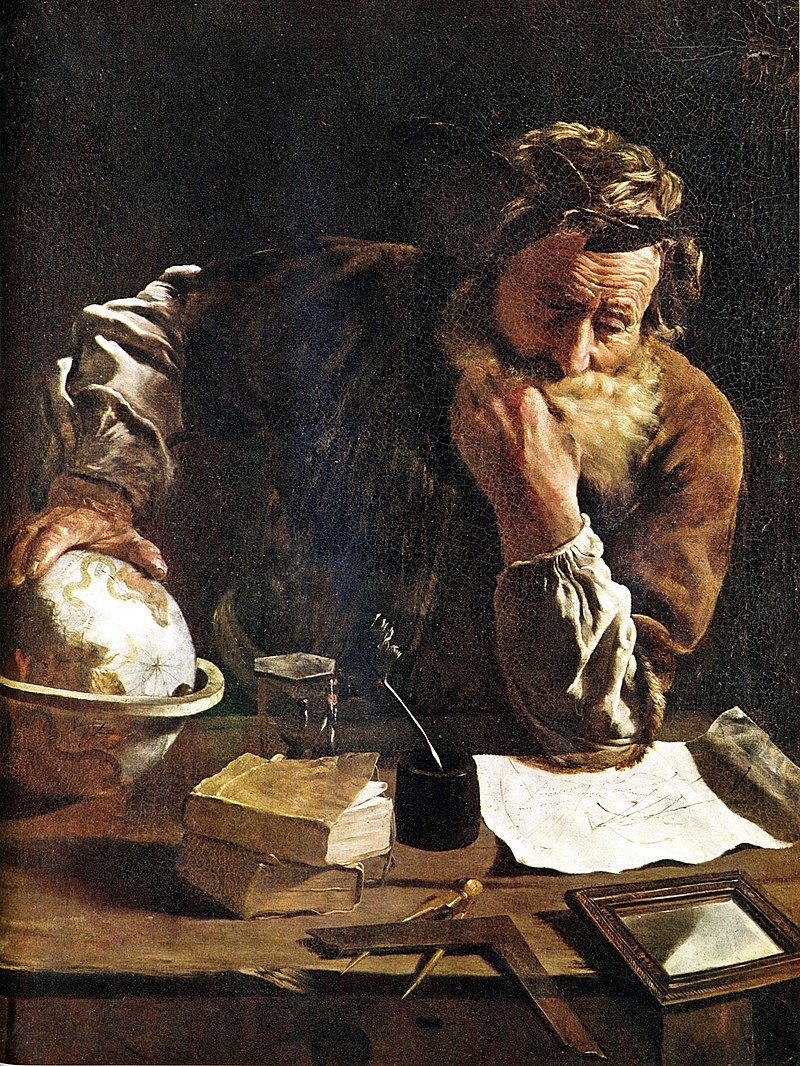
\includegraphics[width=0.5\textwidth,height=\textheight]{images/Domenico-Fetti_Archimedes_1620.jpg}
\caption[Archimedes of Syracuse.]{Archimedes of
Syracuse.\footnotemark{}}\label{fig:archimedes}
\end{figure}
\footnotetext{Domenico Fetti's 1620 painting entitled \emph{Archimedes
  Thoughtful}. Public domain.}

Among the many accomplishments of Archimedes is his method for
estimating \(\pi\), which was the best approximation for almost 1900
years. And it was not based on using a length of string, superimposing
it on a circle, and getting an estimate! \emojifont {😉}\normalfont 

What is even more remarkable is that Archimedes made his discovery
\emph{without} the benefit of:

\begin{enumerate}
\def\labelenumi{(\alph{enumi})}
\item
  the real numbers;
\item
  algebra;
\item
  trigonometry;
\item
  decimal notation; and
\item
  devices like logarithm tables, slide rules, calculators, or computers.
\end{enumerate}

Instead he applied geometry---including the theorem of Pythagoras---and
extracted rational values for square roots, laboriously by hand. His
method is also an excellent geometrical illustration of the idea of a
\href{https://www.britannica.com/science/limit-mathematics}{\emph{limit}},
with which he was doubtless familiar. It is known that Archimedes was
familiar with what we now know as integral calculus, and it is possible
that he may have anticipated differential calculus as well.

Archimedes devised an ingenious method for estimating the circumference
of a circle. He used a simple yet sophisticated algorithm that allowed
him to obtain successively more accurate values for the circumference of
a circle, and therefore of \(\pi\).

\begin{figure}
\centering
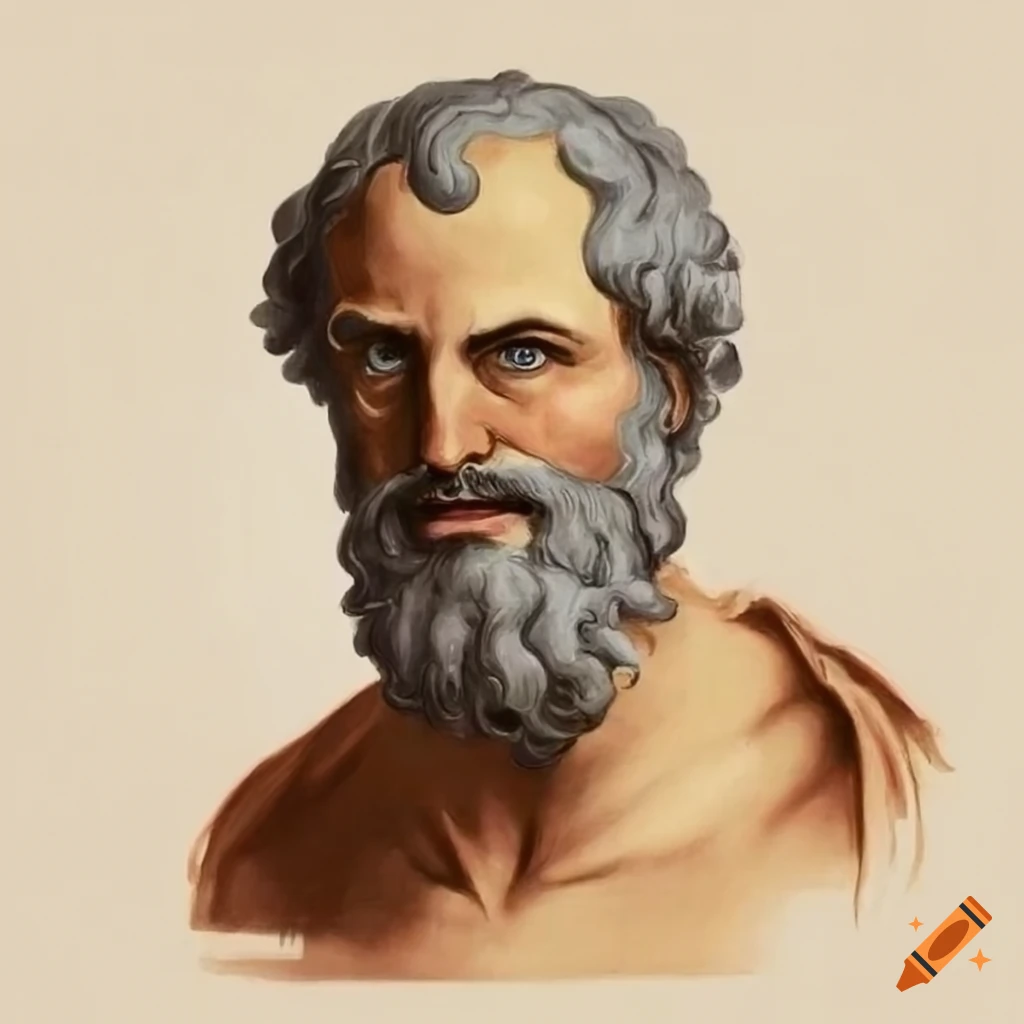
\includegraphics[width=0.7\textwidth,height=\textheight]{images/Archimedes-AI-generated-portrait.png}
\caption{Portrait of Archimedes generated by AI and available at the
Craiyon website
\href{https://www.craiyon.com/image/JEmP4rPCRW25xyCULOeMSw}{here}. All
portraits of Archimedes are flights of fancy rather than true
likenesses.}\label{fig:Archimedes-AI}
\end{figure}

\subsection{Principles used by
Archimedes}\label{principles-used-by-archimedes}

The method that Archimedes devised is instructive because it is a
synthesis of several principles by which the greatest human minds have
furthered scientific progress over time. The abstract principles that
Archimedes used to estimate \(\pi\) were these:

\begin{enumerate}
\item
  Start with the known and progress to the unknown;
\item
  Initialize variables;
\item
  Devise a method of increasing the accuracy of the estimate by
  \href{https://mathworld.wolfram.com/Recursion.html}{recursion} or
  \href{https://www.vocabulary.com/dictionary/iteration}{iteration};
\item
  Stop when the desired accuracy is reached.
\end{enumerate}

These principles constitute what is known as an
\href{https://www.merriam-webster.com/dictionary/algorithm}{algorithm}.
Once such a systematic framework has been put in place, it can be
applied in many research domains to aid rapid scientific progress. The
algorithm is the basis of modern computing.

\subsection{Of polygons and circles}\label{of-polygons-and-circles}

Archimedes considered a circle, containing an
\href{https://mathworld.wolfram.com/Inscribed.html}{inscribed} regular
polygon with \(n\) sides, and
\href{https://mathworld.wolfram.com/Circumscribed.html}{circumscribed}
by a regular polygon with the same \(n\) sides. \cref{fig:two-limits}
illustrates this for the case \(n = 6\), i.e., with a regular
\href{https://www.britannica.com/science/hexagon}{hexagon}.

\begin{figure}
\centering
\includesvg[width=0.7\textwidth,height=\textheight]{images/two-limits.svg}
\caption{The circumference of the circle in darkolivegreen is bounded
from below by the perimeter of the inscribed regular hexagon in maroon
and bounded from above by the perimeter of the circumscribed regular
hexagon in midnightblue. The circumference of the circle must lie
between the perimeters of these two hexagons. The value \(r\) is the
radius of the circle and the height \(h\)---from the centre to the
mid-point of a side---is called the
\href{https://en.wikipedia.org/wiki/Apothem}{apothem}.}\label{fig:two-limits}
\end{figure}

\begin{figure}
\centering
\includesvg[width=0.7\textwidth,height=\textheight]{images/sin-theta-tan-theta.svg}
\caption{The relationship between the circle and its inscribed and
circumscribed regular polygons. The symbol \(h\) is used for the apothem
in both cases. Note that \(OD = h = r\cos\theta\) for the inscribed
polygon, whereas \(OC = h = r\) for the circumscribed
polygon.}\label{fig:sin-theta-tan-theta}
\end{figure}

Let us tabulate below the variables arising from
\cref{fig:two-limits,fig:sin-theta-tan-theta}.

\begin{longtable}[]{@{}
  >{\raggedright\arraybackslash}p{(\columnwidth - 6\tabcolsep) * \real{0.1270}}
  >{\raggedright\arraybackslash}p{(\columnwidth - 6\tabcolsep) * \real{0.1746}}
  >{\raggedright\arraybackslash}p{(\columnwidth - 6\tabcolsep) * \real{0.4127}}
  >{\raggedright\arraybackslash}p{(\columnwidth - 6\tabcolsep) * \real{0.2857}}@{}}
\caption{\label{tbl:variables}Circle, inscribed, and circumscribed
regular polygons (\(n\)-gons).}\tabularnewline
\toprule\noalign{}
\begin{minipage}[b]{\linewidth}\raggedright
Parameter
\end{minipage} & \begin{minipage}[b]{\linewidth}\raggedright
Circle
\end{minipage} & \begin{minipage}[b]{\linewidth}\raggedright
Inscribed
\end{minipage} & \begin{minipage}[b]{\linewidth}\raggedright
Circumscribed
\end{minipage} \\
\midrule\noalign{}
\endfirsthead
\toprule\noalign{}
\begin{minipage}[b]{\linewidth}\raggedright
Parameter
\end{minipage} & \begin{minipage}[b]{\linewidth}\raggedright
Circle
\end{minipage} & \begin{minipage}[b]{\linewidth}\raggedright
Inscribed
\end{minipage} & \begin{minipage}[b]{\linewidth}\raggedright
Circumscribed
\end{minipage} \\
\midrule\noalign{}
\endhead
\bottomrule\noalign{}
\endlastfoot
Radius & \(r\) & & \\
Sides & & \(n\) & \(n\) \\
Length & & \(2r\sin\theta\) & \(2r\tan\theta\) \\
Angle & & \(\theta(n) = \frac{\pi}{n} = \frac{180°}{n}\) &
\(\theta(n) = \frac{\pi}{n}=\frac{180°}{n}\) \\
Apothem & & \(h = r\cos\theta\) & \(h = r\) \\
Area & \(A = \pi r^2\) & \(a(n) = n\sin\theta\cos\theta r^2\) &
\(A(n) = n\tan\theta r^2\) \\
Perimeter & \(C = 2\pi r\) & \(c(n) = 2n\sin\theta r\) &
\(C(n) = 2n\tan\theta r\) \\
\end{longtable}

~

When \(n\) varies, so do the values of \(\theta\) and the areas and
perimeters; they are therefore shown as functions of \(n\) in
\cref{tbl:variables}.

\subsection{Recursion and Iteration}\label{recursion-and-iteration}

Archimedes started with regular hexagons and successively \emph{doubled}
the number of sides, until he had the circle closely sandwiched between
two 96-gons---one circumscribed; the other inscribed. Successively
doubling or halving is a fast-converging technique used in numerical
estimation, called the
\href{https://en.wikipedia.org/wiki/Bisection_method}{bisection method},
that is applied to solving a variety of problems. That Archimedes was
aware of it shows how far ahead of his time his thinking was.

When he moved from \(n=6\) to \(n = 12\) sides, how did Archimedes
estimate the respective perimeters without the aid of trigonometry? He
used geometry and the Pythagorean theorem,
\href{https://nonagon.org/ExLibris/archimedes-pi}{as described here
online} {[}\citeproc{ref-bertrand2014}{1}{]}
\href{https://publications.azimpremjiuniversity.edu.in/3356/1/02-DaminiAndAbhishek_PiIs22By7_Final.pdf}{and
here} {[}\citeproc{ref-damini-dhar-2020}{2}{]}to obtain
\href{https://en.wikipedia.org/wiki/Recurrence_relation}{recurrence
relations} that gave the current result from the previous one.

For an English translation of the book \emph{Measurement of a Circle} by
Archimedes \href{auxiliary/Archimedes-Circle.pdf}{click on this link}.
It is the original source material from the man himself, and will give
you a sense of completeness in your understanding of his method.

He repeatedly calculated \emph{rational approximations} to \(\pi\) until
he was satisfied with the accuracy. The principle of the method is
clearly seen in
\cref{fig:six-gon,fig:twelve-gon,fig:twenty-four-gon,fig:forty-eight-gon,fig:ninety-six-gon}.

\begin{figure}
\centering
\includesvg[width=0.7\textwidth,height=\textheight]{images/six-gon.svg}
\caption{The estimate for \(\pi\) lies between
\(C_i = 3.0000 < \pi < C_c = 3.4641\).}\label{fig:six-gon}
\end{figure}

\begin{figure}
\centering
\includesvg[width=0.7\textwidth,height=\textheight]{images/twelve-gon.svg}
\caption{The estimate for \(\pi\) lies between
\(C_i = 3.1058 < \pi < C_c = 3.2153\).}\label{fig:twelve-gon}
\end{figure}

\begin{figure}
\centering
\includesvg[width=0.7\textwidth,height=\textheight]{images/twenty-four-gon.svg}
\caption{The estimate for \(\pi\) lies between
\(C_i = 3.1326 < \pi < C_c = 3.1596\).}\label{fig:twenty-four-gon}
\end{figure}

\begin{figure}
\centering
\includesvg[width=0.7\textwidth,height=\textheight]{images/forty-eight-gon.svg}
\caption{The estimate for \(\pi\) lies between
\(C_i = 3.1393 < \pi < C_c = 3.1460\).}\label{fig:forty-eight-gon}
\end{figure}

\begin{figure}
\centering
\includesvg[width=0.7\textwidth,height=\textheight]{images/ninety-six-gon.svg}
\caption{The estimate for \(\pi\) lies between
\(C_i = 3.1410 < \pi < C_c = 3.1427\). Notice in this sequence of images
how the circumference of the circle approaches the perimeter of the
inscribed and circumscribed heaxgons to the point of being
indistinguishable from them. \emph{The final estimate of Archimedes was
\(\frac{223}{71} < \pi < \frac{22}{7}\).}}\label{fig:ninety-six-gon}
\end{figure}

\subsection{Lower and upper bounds for
π}\label{lower-and-upper-bounds-for-ux3c0}

We assume that \(r = 1\) without loss of generality.
\cref{tbl:variables} and \cref{fig:sin-theta-tan-theta} together give us
these inequalities for regular \(n\)-gons where
\(\theta = \frac{180}{n}\) degrees or \(\theta = \frac{\pi}{n}\)
radians. \begin{equation}\phantomsection\label{eq:squeeze}{
\begin{aligned}
a(n) < A < A(n) &\implies n\sin\theta\cos\theta < \pi < n\tan\theta\\
c(n) < C < C(n) &\implies n\sin\theta < \pi < n\tan\theta
\end{aligned}
}\end{equation}

From the right hand side of \cref{eq:squeeze}, using the inequalities
for perimeters, we have
\begin{equation}\phantomsection\label{eq:lower-bound}{
n\sin\tfrac{180°}{n} = n\sin\tfrac{\pi}{n}, \thinspace \mbox{for the lower bound}.
}\end{equation} \begin{equation}\phantomsection\label{eq:upper-bound}{
n\tan\tfrac{180°}{n} = n\tan\tfrac{\pi}{n}, \thinspace \mbox{for the lower bound}.
}\end{equation}

\cref{eq:lower-bound,eq:upper-bound} represent respectively the lower
and upper bounds on the value of \(\pi\) obtained through the method of
Archimedes.

Obviously, the circle may be viewed as a regular polygon whose number of
sides, \(n\) has become exceedingly large, or \emph{infinite}. So, as
\(n\) is increased, we should expect the two bounds to converge to the
limiting value of \(\pi\).

\begin{longtable}[]{@{}lll@{}}
\caption{\label{tbl:large-n-pi}The values of \(n\sin\frac{\pi}{n}\) and
\(n\tan\frac{\pi}{n}\). As \(n\) larger and larger, the values in both
the second and third columns become closer and closer to
\(\pi\).}\tabularnewline
\toprule\noalign{}
\(n\) & \(n\sin\frac{\pi}{n}\) & \(n\tan\frac{\pi}{n}\) \\
\midrule\noalign{}
\endfirsthead
\toprule\noalign{}
\(n\) & \(n\sin\frac{\pi}{n}\) & \(n\tan\frac{\pi}{n}\) \\
\midrule\noalign{}
\endhead
\bottomrule\noalign{}
\endlastfoot
\(6\) & \(3.0000000000\) & \(3.4641016151\) \\
\(12\) & \(3.1058285412\) & \(3.2153903092\) \\
\(24\) & \(3.1326286133\) & \(3.1596599421\) \\
\(48\) & \(3.1393502030\) & \(3.1460862151\) \\
\(96\) & \(3.1410319509\) & \(3.1427145996\) \\
\(100\) & \(3.1410759078\) & \(3.1426266043\) \\
\(1000\) & \(3.1415874859\) & \(3.1416029891\) \\
\(10000\) & \(3.1415926019\) & \(3.1415927569\) \\
\(100000\) & \(3.1415926531\) & \(3.1415926546\) \\
\(1000000\) & \(3.1415926536\) & \(3.1415926536\) \\
\end{longtable}

~

The upper and lower bounds are equal up to ten decimal digits when
\(n = 10^{6}\), and we might declare the problem of estimating pi
solved. But in the time of Archimedes, trigonometry was not known; only
geometry was. Moreover, the decimal system and calculators were also in
the future. We now have to backtrack and attempt to retrace the steps
Archimedes used to estimate \(\pi\).

\subsubsection{The thirty, sixty, ninety right
triangle}\label{the-thirty-sixty-ninety-right-triangle}

Archimedes applied the principle ``of starting from the known'' to
initiate his algorithm using a \emph{regular hexagon}, which is a mosaic
of six juxtaposed equilateral triangles. We know from symmetry that each
angle of an equilateral triangle is \(60°\). When an equilateral
triangle is bisected, we get two right-angled triangles with angles of
thirty and sixty degrees, as shown in \cref{fig:thirty-sixty}.

\begin{figure}
\centering
\includesvg[width=0.7\textwidth,height=\textheight]{images/thirty-sixty.svg}
\caption{This right-angled, obtained by bisecting an equilateral
triangle, must be familiar to all school students. These
lengths---obtainable from symmetry and the theorem of
Pythagoras---allowed Archimedes to start off his process for estimating
\(\pi\).}\label{fig:thirty-sixty}
\end{figure}

The inscribed hexagon, within a circle of radius one unit, also has a
side of one unit. Thus, the hypotenuse of the circle \(OAP\) in
\cref{fig:thirty-sixty} has unit length. Moreover, the base \(OP\),
resulting from a bisected side, has a length of half a unit. By applying
the theorem of Pythagoras, the third side, \(AP\) is
\begin{equation}\phantomsection\label{eq:triangle}{
\sqrt{1^2 - \left(\frac{1}{2}\right)^2} = \frac{\sqrt{3}}{2}.
}\end{equation}

The next thing Archimedes needed and knew how to do was to compute
\(\sqrt{3}\) which figures in \cref{eq:triangle}. Finding square roots
is a tedious process, not unlike long division, and prone to human
error. The patience and doggedness of Archimedes that must have gone
into the process is astounding.

\subsubsection{Extracting square roots by
hand}\label{extracting-square-roots-by-hand}

Archimedes must have known how to extract square roots by hand. Perhaps,
he used one of the methods described in my blog
\href{https://swanlotus.netlify.app/blogs/how-are-numbers-built}{``How
Are Numbers Built?''}. He should have known the value of \(\sqrt{3}\) as
a rational fraction. With remarkable accuracy, he stated that:
\begin{equation}\phantomsection\label{eq:sqrt3}{\sqrt{3} \approx \frac{265}{153} \approx 1.732.
}\end{equation}

\subsection{Trigonometry and half
angles}\label{trigonometry-and-half-angles}

Archimedes had no trigonometric tables to aid him. But he did know the
square root of three, and the geometric properties of triangles whose
angles were repeatedly bisected. He used a previous result to feed
values into the next result as he doubled the sides of the regular
hexagon. We will look at his method a little later, but for now, we will
try to simulate what he did using trigonometry. In the process we will
encounter an important ides called
\href{(https://www.geeksforgeeks.org/introduction-to-recursion-2/)}{recursion}
which is a bit like a snake eating its own tail.

From \cref{fig:thirty-sixty}, we know:
\begin{equation}\phantomsection\label{eq:three-six-nine}{
\begin{aligned}
\sin 30° &= \tfrac{1}{2}\\
\cos 30° &= \tfrac{\sqrt{3}}{2}\\
\tan 30° &= \tfrac{\sqrt{3}}{3}\\
\end{aligned}
}\end{equation}

\subsection{The half-angle formulae and
recursion}\label{the-half-angle-formulae-and-recursion}

The whole trick to this recursion is to

\begin{enumerate}
\item
  move from one estimate to the next, more accurate estimate of \(\pi\);
  and
\item
  use one known value of a trigonometric function to estimate the next
  unknown value in the chain.
\end{enumerate}

The trigonometry of
\href{https://math.libretexts.org/Bookshelves/Algebra/Algebra_and_Trigonometry_1e_(OpenStax)/09:_Trigonometric_Identities_and_Equations/9.03:_Double-Angle_Half-Angle_and_Reduction_Formulas}{half
angles in terms of the full angle} {[}\citeproc{ref-half-angle}{3}{]}
helps relate the successive values of \(\theta\):\footnote{All angles
  are in the first quadrant.} \[
\begin{aligned}
\sin\frac{\theta}{2} = \sqrt{\frac{1 - \cos\theta}{2}}\\
\cos\frac{\theta}{2} = \sqrt{\frac{1 + \cos\theta}{2}}\\
\end{aligned}
\]

Let us step through the recursion:

\begin{enumerate}
\item
  We know from \cref{fig:thirty-sixty} that \(\sin 30° = \frac{1}{2}\)
  and \(\cos 30° = \frac{\sqrt{3}}{2}\).
\item
  We calculate \(\sin 15°\) etc., from \(\cos 30°\) using the half-angle
  formula: \[
  \begin{aligned}
  \sin 15° &= \sqrt{\frac{1 - \frac{\sqrt{3}}{2}}{2}}\\
  &= \sqrt{\frac{2 - \sqrt{3}}{4}}\\
  &= \frac{1}{2}\sqrt{2 - \sqrt{3}}\\
  \cos 15° &= \sqrt{\frac{1 + \frac{\sqrt{3}}{2}}{2}}\\
  &= \sqrt{\frac{2 + \sqrt{3}}{4}}\\
  &= \frac{1}{2}\sqrt{2 + \sqrt{3}}\\
  \tan 15° &= \frac{\sqrt{2 - \sqrt{3}}}{\sqrt{2 + \sqrt{3}}}\\
  \end{aligned}
  \]
\item
  Using the value of \(\cos 15°\), for \(7.5°\) we get \[
  \begin{aligned}
  \sin 7.5° &= \sqrt{\frac{1 - \frac{1}{2}\sqrt{2 + \sqrt{3}}}{2}}\\
  &= \frac{1}{2}\sqrt{2 - \sqrt{2 + \sqrt{3}}}\\
  \cos 7.5° &= \sqrt{\frac{1 + \frac{1}{2}\sqrt{2 + \sqrt{3}}}{2}}\\
  &= \frac{1}{2}\sqrt{2 + \sqrt{2 + \sqrt{3}}}\\ 
  \end{aligned}
  \]
\item
  Using the value of \(\cos 7.5°\), for \(3.75°\) we get: \[
  \begin{aligned}
  \sin 3.75° &= \sqrt{\frac{1 - \frac{1}{2}\sqrt{2 + \sqrt{2 + \sqrt{3}}}}{2}}\\
  &= \frac{1}{2}\sqrt{2 - \sqrt{2 + \sqrt{2 + \sqrt{3}}}}\\
  \cos 3.75° &= \frac{1}{2}\sqrt{2 + \sqrt{2 + \sqrt{2 + \sqrt{3}}}}\\
  \end{aligned}
  \]
\item
  We can see a pattern emerge and we \emph{guess} that the values for
  \(\theta = 1.875°\) corresponding to \(n=96\) \emph{should} be: \[
  \begin{aligned}
  \sin 1.875° &= \frac{1}{2}\sqrt{2 - \sqrt{2 + \sqrt{2 + \sqrt{2 + \sqrt{3}}}}}\\
  \cos 1.875° &= \frac{1}{2}\sqrt{2 + \sqrt{2 + \sqrt{2 + \sqrt{2 + \sqrt{3}}}}}\\
  \end{aligned}
  \] Because we guessed, we checked the value we obtained
  above---expressed as a decimal---with a calculator, and it checked
  out.
\end{enumerate}

We went through this somewhat painful process for the reasons outlined
below because we wanted to simulate the steps Archimedes took
{[}{[}\citeproc{ref-damini-dhar-2020}{2}{]}; bertrand2014{]}. It is a
proof of concept where we have only evaluated the sine and cosine values
and not estimated the two perimeters.

\begin{enumerate}
\def\labelenumi{(\alph{enumi})}
\item
  Archimedes knew the sine of 30° and had to work out all other values
  by hand, without using decimals. That was why we started with a
  regular hexagon and retained \href{}{surds}, along with their awkward
  algebraic manipulation.
\item
  Archimedes only knew \href{}{rational numbers} of the form
  \(\frac{a}{b}\) where \(a\) and \(b\) are integers and \(b \neq 0\).
  So, his approximations for \(\sqrt{2}\) and \(\sqrt{3}\) were
  expressed as improper fractions that approximated those numbers.
\item
  Archimedes did not have positional notation for his calculations and
  he had to rely on an arithmetical system that we would find
  forbidding.
\item
  We have demonstrated how Archimedes used recursion in his estimate of
  \(\pi\).
\item
  We cheated when we used trigonometric half-angle formulae. Archimedes
  did not have those but he used triangles in a semi-circle and
  leveraged his knowledge of similar triangles and Pythagoras's theorem
  because the angle in a semi-circle is a right angle. We use a slightly
  different approach, considered next, to get the results he did,
  without using trigonometry.
\end{enumerate}

\subsubsection{The angle bisector
theorem}\label{the-angle-bisector-theorem}

Without using the half-angle formulae of trigonometry, how can we
successively obtain expressions for the values of \(c(n)\) and \(C(n)\)
as we halve the angles and double the sides each time? We have to rely
on something called the
\href{https://en.wikipedia.org/wiki/Angle_bisector_theorem}{angle
bisector theorem} from geometry.

This derivation might seem tedious, but it is closer to what Archimedes
did in order to establish the recurrence relation that tied the current
value to the previous value.

\begin{figure}
\centering
\includesvg[width=0.7\textwidth,height=\textheight]{images/angle-bisector.svg}
\caption{The angle bisector theorem. The relative lengths of the two
segments that a triangle's side is divided into by a line that bisects
the opposite angle equals the relative lengths of the other two sides of
the triangle, as shown on the diagram.}\label{fig:angle-bisector}
\end{figure}

Referring to \cref{fig:angle-bisector}, if the line \(OC\) bisects the
angle \(BOA\), then the base \(AB\) is divided in the same ratio as the
corresponding sides. This means
\begin{equation}\phantomsection\label{eq:angle-bisector}{
\begin{aligned}
\frac{AO}{OB} &= \frac{AC}{CB} \mbox{ which in turn means that }\\
\frac{a}{b} &= \frac{p}{q}\\
\end{aligned}
}\end{equation}

Applying the theorem to a thirty-sixty-ninety right-angled triangle, we
get \cref{fig:bisect-thirty} shown below.

\begin{figure}
\centering
\includesvg[width=0.45\textwidth,height=\textheight]{images/bisect-thirty.svg}
\caption{The angle bisector theorem applied to a thirty-sixty-ninety
right triangle. The ratio of \(a\) to \(b\) is that same as the ratio of
\(2\) to \(\sqrt{3}\).}\label{fig:bisect-thirty}
\end{figure}

\subsubsection{Numerical results}\label{numerical-results}

WHERE TO PUT THIS?

Evaluating the bounds given in \cref{tbl:variables} and
\cref{eq:squeeze} by setting \(r = 1\), \(n = 6\), and
\(\theta = \frac{180}{n} = 30°\)\footnote{Rather than use radians with
  \(\pi\) entering the proceedings, I decided to stick with degrees as
  units to avoid confusion. If one uses power series to probe further,
  of course, radians are called for.} gives us these values:
\begin{equation}\phantomsection\label{eq:triple-6}{
\begin{aligned}
C_i &= 2n\sin\theta r = 12(\sin 30°) = 12(0.5) &= 6.0000.\\
C &= 2\pi r &= 6.2381.\\
C_c &= 2n\tan\theta r = 12(\tan 30°) = 12\left(\tfrac{\sqrt{3}}{3}\right) = 4\sqrt{3} &\approx 6.9282.\\
\end{aligned}
}\end{equation}

Archimedes doubled \(n\) four times to compute values for regular
polygons with \(12\), \(24\), \(48\), and \(96\) sides. For his last
calculation with \(n = 96\) and
\(\theta = \tfrac{180}{96}° \approx 1.875°\), we have:
\begin{equation}\phantomsection\label{eq:triple-96}{
\begin{aligned}
C_i &= 2n\sin\theta r = 2(96)\sin{1.875°} \approx 192(0.0327) &\approx 6.2820.\\
C &= 2\pi r &= 6.2381.\\
C_c &= 2n\tan\theta r = 2(96)\tan{1.875°} \approx 192(0.0327) &\approx 6.2854.\\
\end{aligned}
}\end{equation}

Note that in the case of 96 sides, we have a \emph{very small angle}
\(\theta\) whose \(\sin\) and \(\tan\) are almost equal. This is what
gives us tight bounds on the estimate of \(\pi\). If you know the power
series for \(\sin\theta\) and \(\tan\theta\), you will appreciate even
better how the value of \(\pi\) is trapped and squeezed between these
two rather close limits.

Remember \cref{eq:triple-96} because it helps us to estimate lower and
upper bounds for the value of the circumference. Archimedes's
application of the
\href{https://en.wikipedia.org/wiki/Squeeze_theorem}{squeeze theorem}
nineteen centuries before the calculus was invented is illustrated in
the series of figures,
\cref{fig:six-gon,fig:twelve-gon,fig:twenty-four-gon,fig:forty-eight-gon,fig:ninety-six-gon}.

\href{https://en.wiktionary.org/wiki/sanity_check}{Sanity check}: Does
\(2\pi = 6.2820\), from a calculator, lie within the bounds of
\cref{eq:triple-96}? Yes, indeed, and we are
\href{https://dictionary.cambridge.org/dictionary/english/be-home-and-dry}{home
and dry}.

Second sanity check: When \(n\) is very large, we expect
\(n\sin\frac{180°}{n}\) to be closer and closer to the true value.
Setting \(n = 10^6\) and evaluating on a calculator we get
\(10^6\sin\frac{180°}{10^6} = 3.14159\) which is reassuring. This deep
connection between the circle and the trigonometric functions also
explains why they are sometimes called the \emph{circular functions}.
Indeed, the values \(n\sin\frac{\pi}{n}\) and \(n\sin\tan{\pi}{n}\) both
converge to \(\pi\) for very large \(n\). The interested reader should
plot these two curves.

WHERE SHOULD THIS GO?

Imagine the mathematical
\href{https://www.merriam-webster.com/word-of-the-day/fortitude-2019-11-21}{fortitude}
of Archimedes to
\href{https://www.collinsdictionary.com/dictionary/english/plough-on}{plough
on}---without algebra or trigonometry or the decimal number system---to
establish the value of \(\pi\).

Before we consider numerical results, there are two aspects of the
problem and the approach taken by Archimedes that I wish to discuss.

\section{}\label{section}

\subsection{Is π really 22/7?}\label{is-ux3c0-really-227}

Is \(\pi\) really equal to \(\frac{22}{7}\), as it has been drummed into
our heads at school? We will answer that question later in this blog.

The answer is a qualified ``Yes and no''. Because \(\pi\) is irrational,
it cannot be expressed precisely in a finite number of digits.
Consequently, we use rational approximations, or a decimal
representation at the desired accuracy for \(\pi\). Thanks to
Archimedes, \(\frac{22}{7}\) is a serviceable overestimate for \(\pi\)
that has survived for centuries.

\subsection{A closer look at π as a
number}\label{a-closer-look-at-ux3c0-as-a-number}

Pi is both an
\href{https://en.wikipedia.org/wiki/Irrational_number}{irrational} and a
\href{https://en.wikipedia.org/wiki/Transcendental_number}{transcendental}
number. Let us see what each of these
\href{https://www.merriam-webster.com/dictionary/appellation}{appelations}
mean.

Recurring decimals.

\subsection{To explore further}\label{to-explore-further}

A well-written, accessible article on how Archimedes estimated that
\(\pi\) is approximately \(\frac{22}{7}\) is available online:
\href{https://publications.azimpremjiuniversity.edu.in/3356/1/02-DaminiAndAbhishek_PiIs22By7_Final.pdf}{``How
Archimedes showed that pi is approximately 22 by 7''}. I urge you to
read it.\footnote{This article is all the more remarkable because its
  first author is a Grade 8 student: proof that deep mathematics is not
  beyond the school student.} You will then appreciate for yourselves
how arduous the process must have been in an age without the benefit of:
\#. Trigonometry; he used the theorem of pythagors instead; \#. Algebra;
he used geometry and the ratios of the lengths of well-known triangles;
\#. Decimal numbers for division; he used fractions instead; square
roots by hand; similar and congruent figures; bisection theorems;
exhaustion methods

In
\cref{fig:six-gon,fig:twelve-gon,fig:twenty-four-gon,fig:forty-eight-gon,fig:ninety-six-gon}
below, which illustrate the approach Archimedes took to estimate
\(\pi\), we see very clearly that the perimeter of the \emph{inscribed
polygon} \(c_n\) and the perimeter of the \emph{circumscribed polygon}
\(C_n\) represent respectively the \emph{lower bound} and \emph{upper
bound} of the estimated value of \(\pi\). As the number of sides, \(n\),
of the polygon increases, the estimates become increasingly accurate.

https://publications.azimpremjiuniversity.edu.in/3356/1/02-DaminiAndAbhishek\_PiIs22By7\_Final.pdf

https://azimpremjiuniversity.edu.in/at-right-angles

\subsubsection{How did Archimedes arrive at π =
22/7?}\label{how-did-archimedes-arrive-at-ux3c0-227}

22/7 = 3.142857 142857 142857 (recurring decimal)

\subsection{Formulae involving π}\label{formulae-involving-ux3c0}

\subsection{Quest for the endless digits of
π}\label{quest-for-the-endless-digits-of-ux3c0}

\subsection{Buffon's Needle}\label{buffons-needle}

\subsection{π Trivia}\label{ux3c0-trivia}

\subsection{Web links}\label{web-links}

https://www.pbs.org/wgbh/nova/physics/approximating-pi.html

https://demonstrations.wolfram.com/ArchimedesApproximationOfPi/ John
Tucker ``Archimedes' Approximation of Pi''
http://demonstrations.wolfram.com/ArchimedesApproximationOfPi/ Wolfram
Demonstrations Project Published: March 5 2009

https://math.stackexchange.com/questions/4851929/archimedes-method-to-estimate-pi

http://arxiv.org/pdf/2008.07995

https://mathsciencehistory.com/2019/10/01/archimedes-and-his-pi-the-great-numerical-hope/

https://carmamaths.org/resources/jon/pi-culture.pdf

https://nonagon.org/ExLibris/archimedes-pi

https://www.exploratorium.edu/pi/history-of-pi

https://en.wikipedia.org/wiki/Approximations\_of\_\%CF\%80

https://www.joyofpi.com/

\subsection{Book References}\label{book-references}

\subsection{Web resources}\label{web-resources}

\subsection{Teaser: are of circle half radius multiplied by
circumference.
How?}\label{teaser-are-of-circle-half-radius-multiplied-by-circumference.-how}

\subsection{Appendix: Circumscribed and inscribed polygons of
circle}\label{appendix-circumscribed-and-inscribed-polygons-of-circle}

Archimedes devised his ingenious \emph{squeeze} method for computing the
upper and lower bounds of the perimeter of a circle by computing instead
the perimeters of the polygons that inscribe and circumscribe the
circle. The approximations become more accurate as the number of sides,
\(n\), of the polygon is increased.
\href{https://www.youtube.com/watch?v=_qdnyw5Eb_Y}{This YouTube
presentation} might help you understand the algorithm of Archimedes
better, but remember that he did not have trigonometry to aid him.

\subsection{Acknowledgements}\label{acknowledgements}

The computations for this blog were performed using programs written by
\href{}{Nandakumar Chandrasekhar} in the
\href{https://julialang.org/}{Julia programming Language}. The source
code is available here:

\subsection{Feedback}\label{feedback}

Please \href{mailto:feedback.swanlotus@gmail.com}{email me} your
comments and corrections.

\noindent A PDF version of this article is
\href{./the-pi-of-archimedes.pdf}{available for download here}:

\begin{small}

\begin{sffamily}

\textless https://swanlotus.netlify.app/blogs/the-pi-of-archimedespdf-blog
.pdf\textgreater{}

\end{sffamily}

\end{small}

\section*{References}\label{bibliography}
\addcontentsline{toc}{section}{References}

\phantomsection\label{refs}
\begin{CSLReferences}{0}{0}
\bibitem[\citeproctext]{ref-bertrand2014}
\CSLLeftMargin{{[}1{]} }%
\CSLRightInline{Mike Bertrand. 2014. {Archimedes and Pi}. Ex libris.
Retrieved 5 July 2024 from
\url{https://nonagon.org/ExLibris/archimedes-pi}}

\bibitem[\citeproctext]{ref-damini-dhar-2020}
\CSLLeftMargin{{[}2{]} }%
\CSLRightInline{Damini D B and Abhishek Dhar. 2022. How archimedes
showed that pi is approximately 22 by 7. \emph{{Azim Premji University
At Right Angles}}. Retrieved 2 July 2024 from
\url{https://publications.azimpremjiuniversity.edu.in/3356/1/02-DaminiAndAbhishek_PiIs22By7_Final.pdf}}

\bibitem[\citeproctext]{ref-half-angle}
\CSLLeftMargin{{[}3{]} }%
\CSLRightInline{OpenStax. {Algebra and Trigonometry}. {Double-Angle,
Half-Angle, and Reduction Formulas}. Retrieved 6 July 2024 from
\url{https://math.libretexts.org/Bookshelves/Algebra/Algebra_and_Trigonometry_1e_(OpenStax)/09:_Trigonometric_Identities_and_Equations/9.03:_Double-Angle_Half-Angle_and_Reduction_Formulas}}

\end{CSLReferences}



\end{document}
